\documentclass[Arkitektur/System_main.tex]{subfiles}

\begin{document}
\section{Grænseflader / Protokoller}
I dette afsnit forklares de forskellige grænseflade mellem delsystemerne, samt hvilke brugerdefineret protokoller de bruger. Systemet gør generelt brug af I2C protokollen, hvor RPi'en er 'Masteren' og PSoC enhederne er 'slaves'. 


\subsection{Kommunikation mellem RPi og PSoC enheder}


Systemet gør brug af I2C-protokollen i forhold til kommunikationen mellem RPi, Playerside og BallDispenser. Kommunikationen mellem enhederne starter enten med at RPi'en (MASTER) ønsker at sende noget til Playerside eller BallDispenser (SLAVES) eller hvis en af slaverne sender et interrupt. Interrupts er nødvendigt, da PSoC enhederne er afhængig af RPi'en SCL - dette er grundprincippet for I2C. 

\begin{figure}[H]
    \centering
    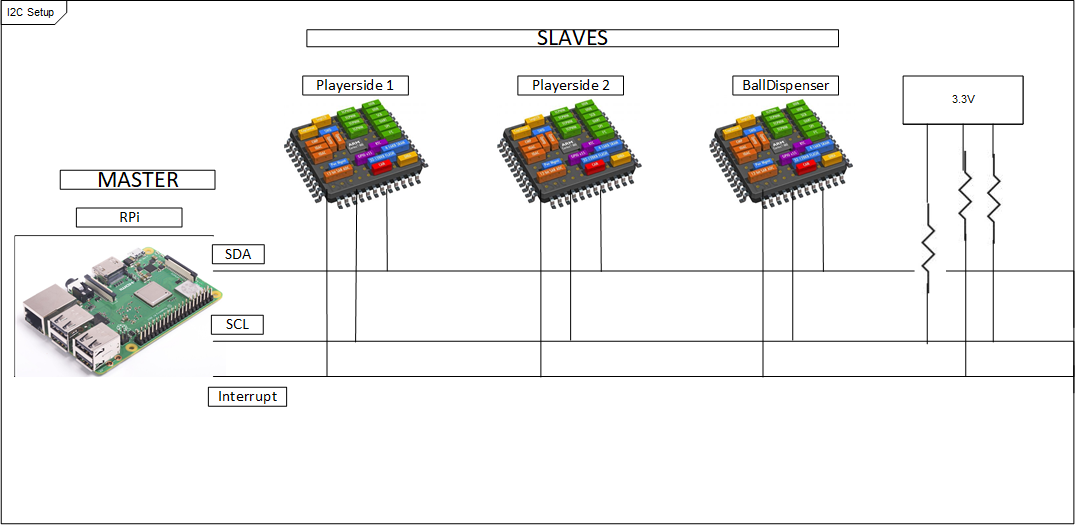
\includegraphics[width=\textwidth]{Arkitektur/Grenseflader/Graphics/I2C.png}
    \caption{Skitse af I2C setup, kommunikation mellem enhederne i systemet}
    \label{fig:i2c_setup}
\end{figure}

\textbf{Interrupts}
\\Mellem RPi'en og de andre enheder eksistere end interruptlinje, som er aktiv lav. Hvis et af delsystemerne, fx en Playerside registrere en fjernelse af kop, sendes et interrupt til RPi ved at "holde" interruptlinjen lavt. Da alle enheder er på samme interruptlinje, anmoder RPi'en hver enhed om 1 byte af data.


\begin{table}[H]
\centering
\begin{tabular}{|l|l|l}
\cline{1-2}
Interruptlinje & Kommando (Binær) &  \\ \cline{1-2}
Data Ready & 00000000 &  \\ \cline{1-2}
No Data & 11111111 &  \\ \cline{1-2}
\end{tabular}
\end{table}
Når denne data er blevet sendt, skal enheden trække linjen højt igen. Hvis et af de andre PSoC enheder stadig trækker linjen lavt, vil RPi'en fortsat anmode om data. Hvis den modtager et "No Data"-byte vil den gå videre og anmode det næste device. 
\\\\\textbf{Eksempel på kommunikation}
\begin{table}[H]
\resizebox{\textwidth}{!}{%
\begin{tabular}{|l|l|l|l|l|l|l|l|l|l|}
\hline
\textbf{Bit 0 - 6} & \textbf{Bit 7} & \textbf{Bit 8} & \textbf{Bit 9 - 16}  & \multicolumn{4}{l|}{\textbf{Bit 17}} \\ \hline
Slave Address & R/W & ACK & Data Bit & \multicolumn{4}{l|}{NACK} \\ \hline
\end{tabular}%
}
\end{table}
\textbf{Slave Address:} Adresse for den PSoC vi ønsker at kommunikere med. \\
\textbf{R/W:} Bit som determinere om RPi'en skal læse eller skrive til en slave \\
\textbf{ACK:} Konfirmation fra slave, at kommando er modtaget. \\
\textbf{Data Bits:} Data som skal sendes eller modtages\\
\textbf{NACK:} Signal i forhold til kommunikation er færdig \\

\begin{table}[H]
\resizebox{\textwidth}{!}{%
\begin{tabular}{|l|l|l|}
\hline
\textbf{Enhed} & \textbf{Adresse (Hex)} & Adresse (Binær) \\ \hline
Playerside 1 & 0x10 & 0010000 \\ \hline
Playerside 2 & 0x11 & 0010001 \\ \hline
BallDispenser & 0x12 & 0010010 \\ \hline
\end{tabular}%
}
\end{table}

\subsubsection{Grænseflade mellem RPi og Playerside}
%Kort introduktion...

\textbf{RPi til Playerside}
\\Kommandoer mellem RPi og Playerside. RPi kontrollerer hvilken stadie Playerside af i via I2C protokollen: 
\begin{table}[H]
\resizebox{\textwidth}{!}{%
\begin{tabular}{|l|l|l|}
\hline
\textbf{RPi til Playerside} & \textbf{Kommando (Hex)} & \textbf{Kommando (Binær)} \\ \hline
\textbf{IDLE} & 0x0A & 00001010 \\ \hline
\textbf{STARTING} & 0x0B & 00001011 \\ \hline
\textbf{PLAYING} & 0x0C & 00001100 \\ \hline
\textbf{LOST} & 0x0D & 00001101 \\ \hline
\textbf{WON} & 0x0E & 00001110 \\ \hline
\end{tabular}%
}
\end{table}

\textbf{Playerside til RPi}
\\Playersides hoved funktion er at sende antal kopper tilbage på de angivede pladser. Denne information er vital for RPi'en, som videregiver denne information til andre delsystemet (fx Display og WebPage). 
Playerside sender en byte til RPi, hvor de 6 LSB bit repræsenterer en kop. Et højt bit betyder at en kop er placeret på den angivet plads osv (se figur \ref{fig:cups_setup}). 
\begin{table}[H]
\centering
\begin{tabular}{lll}
\hline
\multicolumn{1}{|l|}{\textbf{Playerside til RPi}} & \multicolumn{2}{l|}{\textbf{Kommando (Binær)}} \\ \hline
\multicolumn{1}{|l|}{Kopper} & \multicolumn{2}{l|}{00000000} \\ \hline
\multicolumn{3}{l}{}
\end{tabular}
\end{table}

\begin{figure}[H]
    \centering
    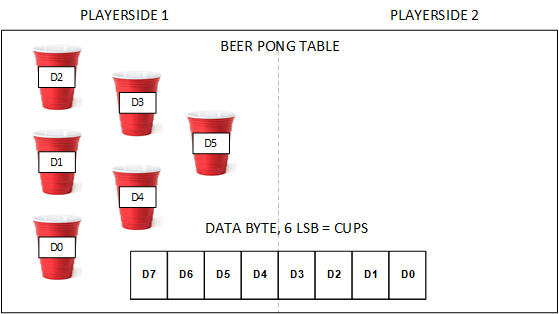
\includegraphics[width=\textwidth]{Arkitektur/Grenseflader/Graphics/cups.png}
    \caption{Repræsentation af 1 byte af kopper}
    \label{fig:cups_setup}
\end{figure}

\subsubsection{Grænseflade mellem RPi og BallDispenser}
Ligesom for Playerside, så kontrollerer RPi'en hvilke stadie BallDispenseren er i. BallDispenseren sender events tilbage til RPi'en: Ingen bolde og Møntindkast. 

\textbf{RPi til BallDispenser}
Kommandoer som indleder tilstandene for BallDispenser. 

\begin{table}[H]
\resizebox{\textwidth}{!}{%
\begin{tabular}{|l|l|l|}
\hline
\textbf{RPi til BallDispenser} & \textbf{Kommando (Hex)} & \textbf{Kommando (Binær)} \\ \hline
Dispense\_On & 0x14 & 00010100 \\ \hline
Dispense\_Off & 0x15 & 00010101 \\ \hline
\end{tabular}%
}
\end{table}

\textbf{BallDispenser til RPi}
Eventbaserede "interrupts" som signaleres til RPi'en fra BallDispenseren. 
\begin{table}[H]
\resizebox{\textwidth}{!}{%
\begin{tabular}{|l|l|l|}
\hline
\textbf{BallDispenser to RPi} & \textbf{Kommando (Hex)} & \textbf{Kommando (Binær)} \\ \hline
CoinInsterted & 0x1E & 00011110 \\ \hline
Empty & 0x1F & 00011111 \\ \hline
NotEmpty & 0x20 & 00100000 \\ \hline
\end{tabular}%
}
\end{table}






\end{document}